In this section, the results of the successfuly implemented methods that perform better will be shown. That means the combination of preconditioning filters and the TDE algorithm and their parameters.

\subsection{Prefiltering methods}
First, as it is a crucial step, the prefiltering methods are assessed individually.

\subsubsection{PNR}

  \begin{figure}[htb]
	  \begin{center}
		  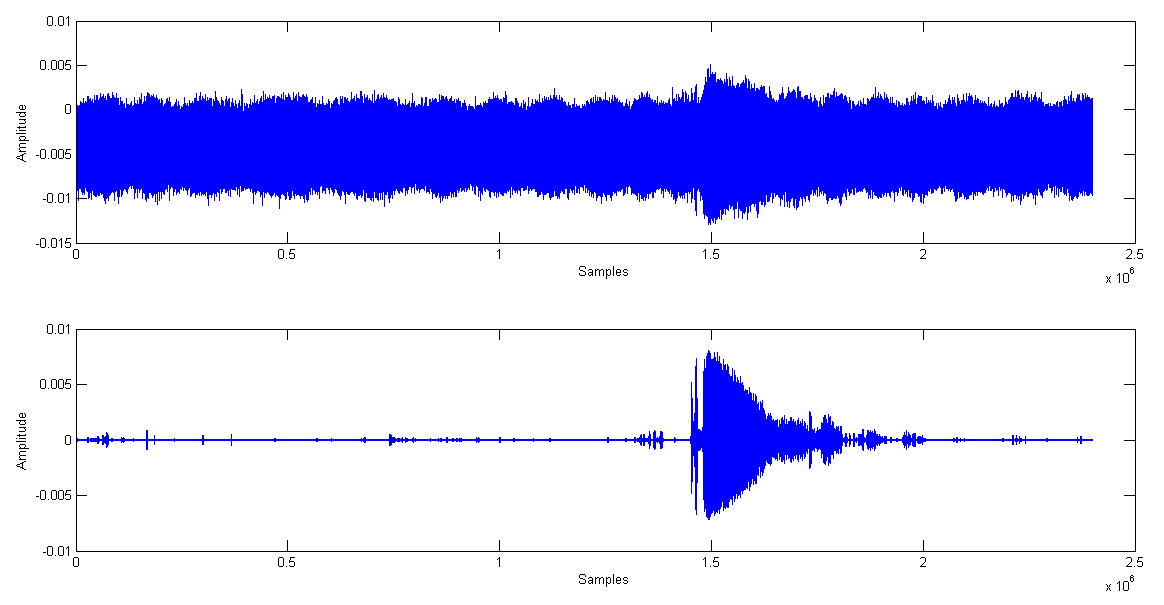
\includegraphics[width=0.5\textwidth]{figures/1PNR_waveform.png}
	  \end{center}
	  \caption{Above: Waveform of sensor 1 recording without pre-processing. Below: Waveform of sensor 1 recording after filter + PNR}
	  \label{fig:result_PNR_waveform}
  \end{figure}

  In the Figure \ref{fig:result_PNR_waveform}, at the top we can see the noisy signal and at the bottom the signal after being processed with Percentile Noise removal. We can observe that the algorithm has deleted almost all of the noise. However, the signal has decreased its level.

  After assessing the improvement, we can state that the SNR before the pre-processing was \SI{3.06}{\dB} and after applying the band pass filter and PNR, it increased up to \SI{39.50}{\dB}. This leads to a good noise reduction algorithm. Computing the entropy, the result is that after the pre-processing the entropy value increases. This is not what we would have expected a priori. The reason is that we have subtracted the correlated noise and pre-whitened the signal. Therefore, we have added a little randomness in the final signal. That is why entropy is not always a good assessment method. However, visually it enhances a lot the scenario and the TDE performs with much more accuracy.
  
  \begin{figure}[htb]
	  \begin{center}
		  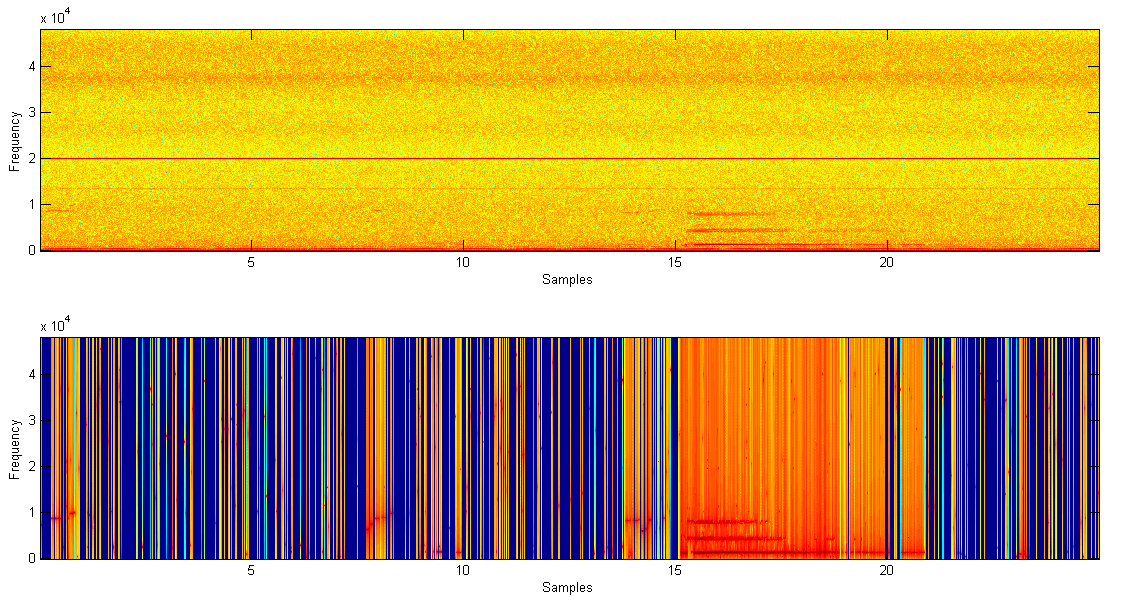
\includegraphics[width=0.5\textwidth]{figures/2PNR_spec.png}
	  \end{center}
	  \caption{Above: Spectrogram of sensor 1 recording without pre-processing. Below: Spectrogram of sensor 1 recording after filter + PNR}
	  \label{fig:result_PNR_spec}
  \end{figure}

  At Figure \ref{fig:result_PNR_spec} we can see the noisy spectrogram and the "clean" spectrogram after being processed with PNR. We can observe that the algorithm has modified completely the Spectrogram. After a lot of work done in the implementation of the algorithm, we could not be able to improve the spectrogram. A missing issue about this algorithm is that there was not enough time to find the optimal parameters: window length and window length shift. This might have improved the visual aspect of the spectrogram. Furthermore, the distance between sensors and the computational complexity of the algorithm made the work harder. However, after simple visual inspection, it's easier to identify the whale sound in the spectrogram, as the SNR of the clean signal has increased.
  

\subsubsection{Spectral Substraction}
  
  \begin{figure}[htb]
	  \begin{center}
		  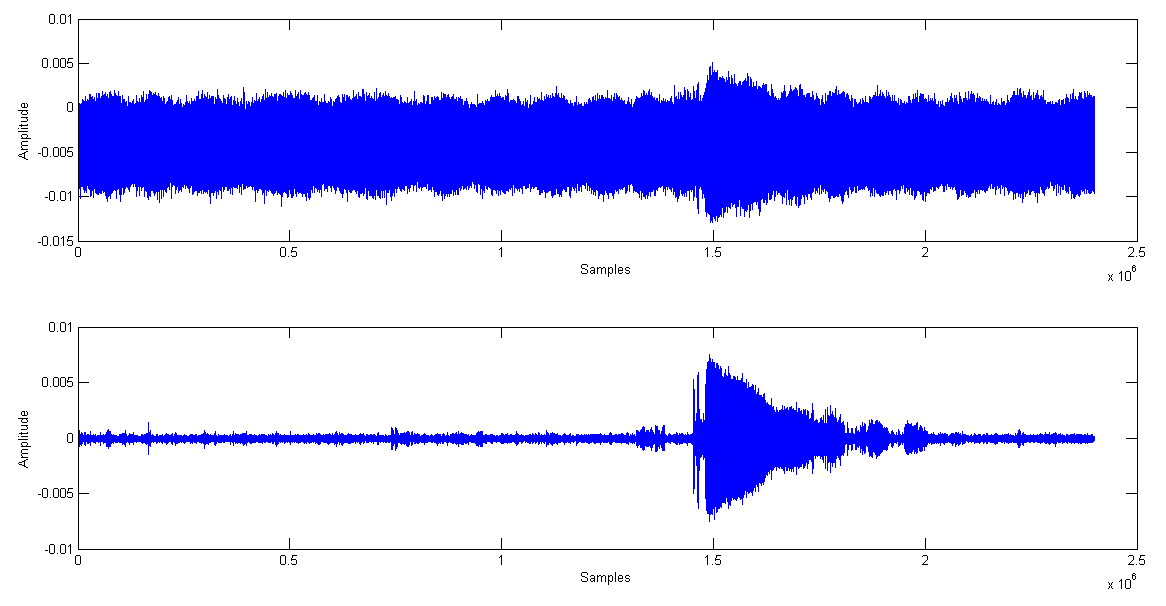
\includegraphics[width=0.5\textwidth]{figures/3SpectralSub_waveform.png}
	  \end{center}
	  \caption{Above: Waveform of sensor 1 recording without pre-processing.  Below: Waveform of sensor 1 recording after filter + Spectral Substraction}
	  \label{fig:result_SS_waveform}
  \end{figure}
  
  Figure \ref{fig:result_SS_waveform} shows the noisy signal and the signal after being processed with Spectral Subtraction. We can observe that the algorithm has deleted most of the noise although the signal has decreased it level a little bit. It doesn't decrease all the noise because of the parameter $\beta$, which fixes a noise floor.
  After assessing the improvement, we can state that the SNR before the pre-processing was \SI{3.0583}{\dB} and after applying the band pass filter + SS, it increased up to \SI{33.88}{\dB}. The same reasoning as in PNR case can be made. The enhancement is a little bit lower but still very high. This is because SS is a particularization of PNR when the percentile value is 50.

  \begin{figure}[htb]
	  \begin{center}
		  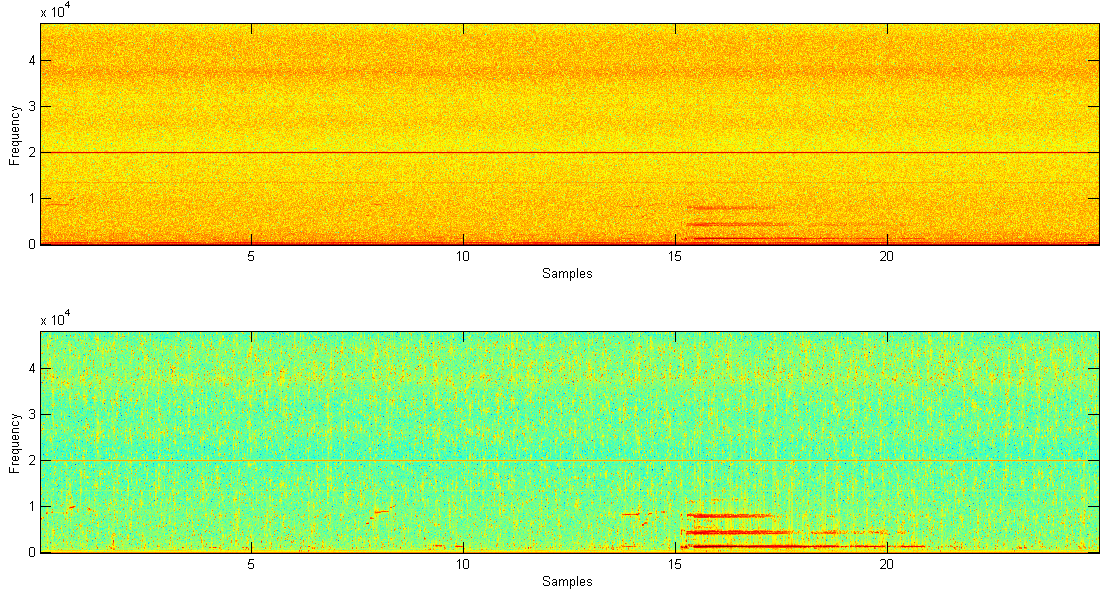
\includegraphics[width=0.5\textwidth]{figures/4SpectralSub_Specgram.png}
	  \end{center}
	  \caption{Above: Spectrogram of sensor 1 recording without pre-processing.  Below: Spectrogram of sensor 1 recording after filter + Spectral Substraction}
	  \label{fig:result_SS_spec}
  \end{figure}
  
  Figure \ref{fig:result_SS_spec} shows the noisy signal and the signal after being processed with Spectral Subtraction. We can observe that the algorithm has a much more good-looking Spectrogram than in PNR method, but the SNR is lower. This could be due to the parameter $\beta$, that allows a little noise level in the clean signal. In TDE, the PNR performs better because, although the clean signal has more distortion, it is looking at the peak to find the correlation between sensors. Then, for our application, we will have better results pre-processing with the PNR rather than with Spectral Subtraction Algorithm.
  
\subsection{TDE}
  With Time Gain Normalization algorithm, we observe quite good results in Time Delay Estimation. All the situations have a relative error below 1\% despite one simulation that has a relative error of 500\% (GCC-SCOT between sensors 1-2. at 2nd Event).
  With Percentile Noise Removal denoising algorithm, the results in Time Delay Estimation outperform. Indeed, all the simulations have a relative error below 0.7\%. If we apply the band-pass filter, we keep obtaining the same results.
  Finally, with Spectral Subtraction algorithm we observe bad results in Time Delay Estimation. Indeed, all the simulations with GCC-PHAT and almost all of them with GCC-SCOT get a relative error of 100\%. If we apply the band pass filter, we keep obtaining good results with the cross-correlation (below 1.5\% of relative error) and we have improved the simulations with PHAT and SCOT. However, PHAT algorithm keep getting a relative error of 50\%.
  As stated before, the cross-correlation algorithm presents good results in all the possible simulations. The interpretation of this results can be understood as the problem of Time Gain Normalization. This is that the high distance between the sensors leads to a small coherence between the received signals, so it makes the PHAT algorithm weak. About the failure of the SCOT without applying the filter can be explained as the Scot algorithm has taken into account the coherence between the strong interference at \SI{20}{\kilo\Hz} in sensors 3 and 4. Then, applying the filter we eliminate that interference.
  We sum up saying that PNR is the best noise reduction algorithm we have explained. We had expected this result when getting \SI{39.5}{\dB} of SNR stated previously.
  
    \subsubsection{GCC-SCOT with PNR}

      \begin{figure}[htb]
	      \begin{center}
		      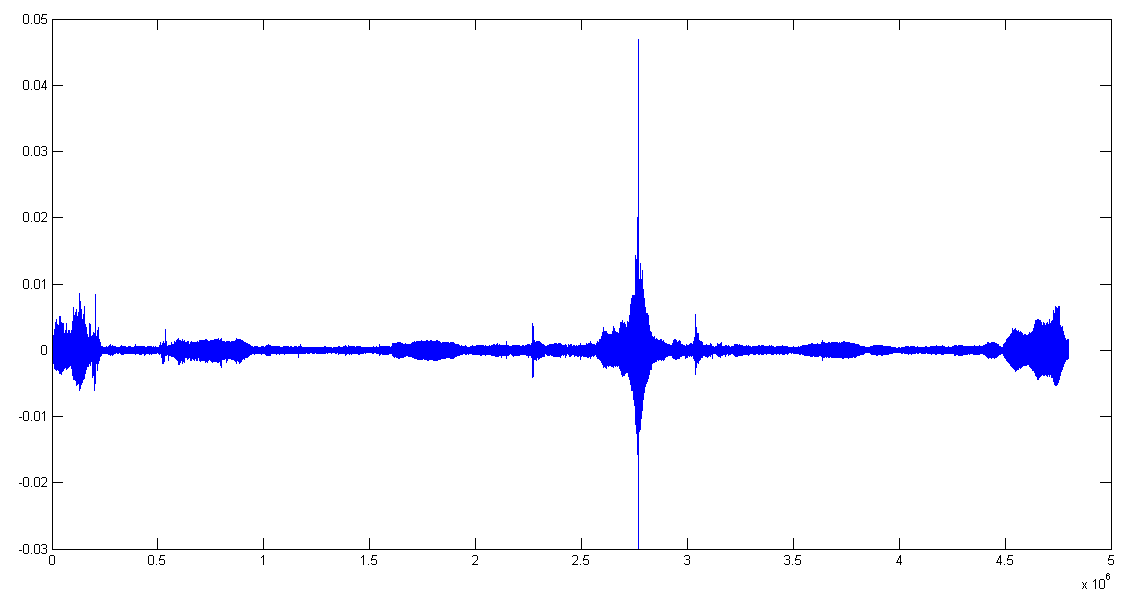
\includegraphics[width=0.5\textwidth]{figures/5gcc_Scot_PNR_12_1.png}
	      \end{center}
	      \caption{GCC-SCOT between sensors 1 and 2 at the first event (2:20-2:45) after PNR}
	      \label{fig:result_GCC_SCOT}
      \end{figure}
      
      Figure \ref{fig:result_GCC_SCOT} shows GCC-SCOT between sensors 1 and 2 at the first minke whale event. As we were expecting after looking at the SNR stated above, the Time Delay Estimation is very accurate. Indeed, we have only a 0.26\% of relative error. GCC-SCOT regularly performs that better. Simulations between sensors 1 and 2, 3, 4 and 5 at the two events and pre-processing with the Percentile Noise Removal algorithm, all of them obtained less than 0.7\% of relative error in all the simulations. We have tried the simulations with these algorithms: Cross-correlation, SCOT Generalised Cross-correlation and PHAT Generalised Cross-correlation.
  
    \subsubsection{GCC-PHAT with Spectral Substraction}
    
    \begin{figure}[htb]
      \begin{center}
	      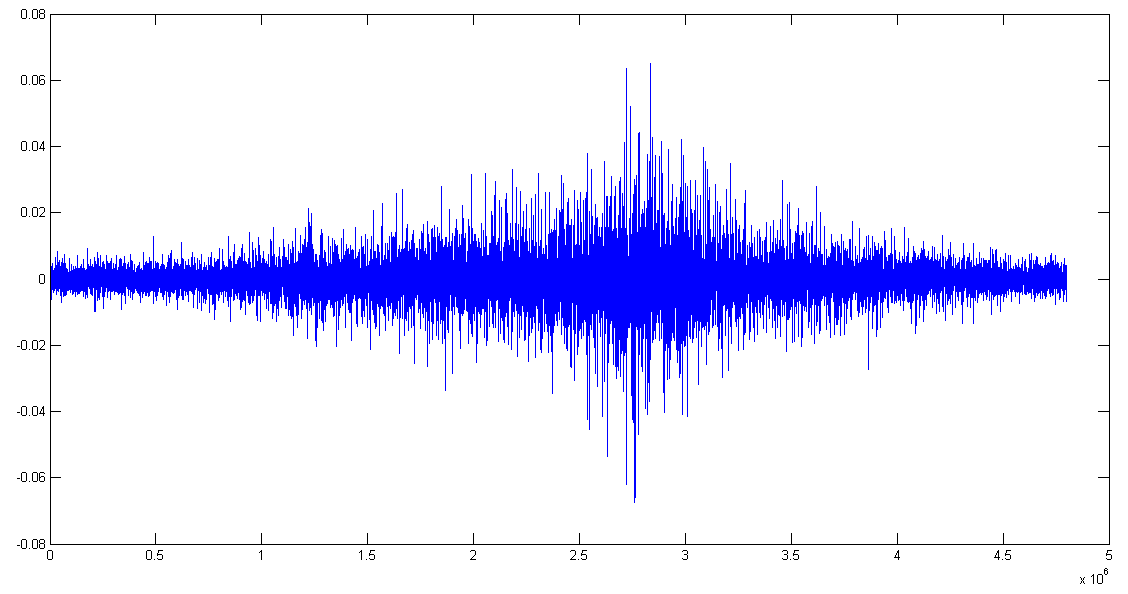
\includegraphics[width=0.5\textwidth]{figures/6gcc_Phat_SS_12_1.png}
      \end{center}
      \caption{GCC-PHAT between sensors 1 and 2 at the first event (2:20-2:45) after Spectral Substraction}
      \label{fig:result_GCC_PHAT}
    \end{figure}
      
    Figure \ref{fig:result_GCC_PHAT} shows GCC-PHAT between sensors 1 and 2 at the first minke whale event. Looking at the plot, we can see that the Time Delay Estimation is quite poor. Indeed, we got relative error of 18\%. PHAT algorithm doesn't work well in all the simulations. Due to the high (12-28 km) distance between the sensors, the coherence of the received signals is very low. While SCOT takes that into account, the PHAT algorithm fails in some of these situations. The PNR is the only noise removal algorithm that leads to a good GCC-PHAT results in all the simulations.
